 %!TEX root = ../dissertation_vkslm.tex

\chapter{Neural Networks and Deep Learning} \label{ch:nndl}
This chapter introduces and gives a brief overview of the theoretical foundations of Deep Neural Networks. In the first section, basic concepts of Artificial Neural Networks are presented, starting from the original models. The next section gives an introduction and a general overview of the deep learning research field, discussing the recent advancements that enabled training Deep Neural Networks successfully. Finally, we briefly describe the fundamentals of the Convolutional Neural Network and present the Fully Convolutional Networks, which is a model used in this work, and we present the techniques used for training our model.

\section{Artificial Neural Networks}

A biological neural network is an essential part of human brain. The human brain is a highly complex information processing system capable of interpreting large amounts of information and making decisions. It is a complex, non-linear and parallel ``computer'' consisting of millions of connected neurons \cite{haykin2009neural}. In many tasks, the human brain is more efficient than computers. For instance, the human brain can recognize a familiar face in about 100-200 ms, while modern computers require minutes or even hours for solving the same problem \cite{haykin2009neural}.

Based on examples and feedback from the ``teacher'', our brain allows us learning how to
distinguish an apple from an orange or recognize letters. Moreover, even without the ``teacher'', we are still able to group similar patterns. Those and other strengths of human brain challenged scientists to emulate those processes by researching how to use machines for tasks that are common for humans. Moreover, one of the concepts that appeared as the result of that research is the Artificial neural network (ANN) concept. 

\subsection{Artificial Neuron}
The first model to simulate a single neuron, which is the elemental building block of neural networks, was the perceptron \cite{rosenblatt1958perceptron}. A single neuron implements a mathematical function given its inputs, to provide an output, as described in Equation \ref{eq:activation} and illustrated in Figure \ref{perceptron}.
\begin{equation}
y = f(\sum_{i=1}^{n} x_{i}w_{i} + b)
\label{eq:activation}
\end{equation}

In this equation, $x_{i}$ is the input $i$, $w_{i}$ is the weight associated with input $i$, $b$ is a
bias term and $f$ the activation function. 
\begin{figure}[!htb]
\centering
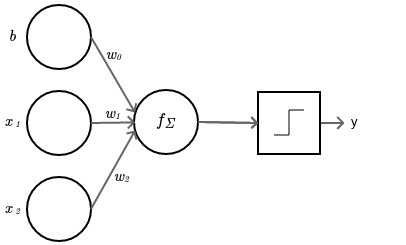
\includegraphics[width=3.4in]{perceptron}
\caption{Perceptron representation. $x_{1}$ and $x_{2}$ represent the input signal, $b$ the bias term, $w_{0}$, $w_{1}$, $w_{2}$ the weights, $f_{\:\sum}$ is the activation function (in this case, a step function) and the output signal is given by $y$.}
\label{perceptron}
\end{figure}

%The learning rule algorithm for learning relations in data with a neuron can be summarized as: for every input $x_{i}$, make a linear prediction about its label: $y^*_{i} = w^T x_{i}$
%and update the weights ($w$) as,
%\begin{equation}
%w \leftarrow w + x_{i}(y_{i} - y^*_{i})
%\end{equation}


Models based on perceptrons have severe limitations. An evaluation by Minsky and Papert \cite{papert1969perceptrons} showed that a perceptron cannot model data that is not linearly separable, such as a simple XOR operator. It was observed that ``for data sets that are not linearly separable, the perceptron learning algorithm will never converge'' \cite{bishop2006pattern}. This observation is related to the perceptron's limited representational power, the learning rule only converges to the correct solution if the data is linearly separable. The Multilayer Perceptron (MLP) with a single hidden layer, however, has been proven \cite{hornik1989multilayer} to approximate any continuous function on a compact input domain to arbitrary precision. For this reason, MLPs are said to be \textit{universal function approximators} \cite{hornik1989multilayer}.

\section{Multi-layer Neural Networks}
Multi-layer Neural Networks such as the MLP consist of stacking several neuron units together. Specifically, in the MLP, neurons are stacked in one layer connecting these stacks sequentially, without connections between the neurons in the same layer, as it is shown in Figure \ref{mlp}. Each neuron in the MLP is normally fully connected with all the neurons in the next layer, with its own set of weights. The first layer of an MLP is usually the input sample, and the last layer is the output of the network. The layers between the input and output layers are called hidden layers.

\begin{figure}[!htb]
\centering
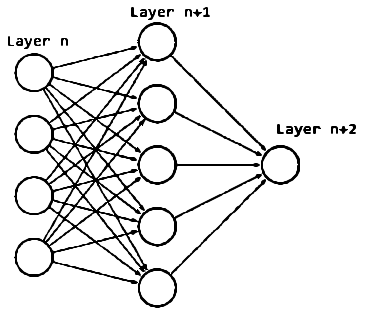
\includegraphics[width=0.8\textwidth]{mlp}
\caption{Multilayer perceptron representation. Each layer contains several perceptron units, which are then connected to units in the subsequent layer.}
\label{mlp}
\end{figure}

An MLP can be thought of as a function that maps from input to output vectors, parameterized by the neuron connection weights. The output of a layer
is calculated by applying the neuron activation function for all neurons on the layer, as
noted in Equation \ref{eq:outputmlp}
\begin{equation}
y^{(l)} = f(W^{(l)} y^{(l-1)} + b^{(l)})
\label{eq:outputmlp}
\end{equation}
where $W^{(l)}$ is a matrix of weights assigned to each pair of neurons from layer $l$ and $l-1$, and $b^{(l)}$ is a vector of bias terms for each neuron in layer $l$. Calculating the output starting from the first hidden layer, up to the output layer is also referred to as the \textit{forward propagation} phase.

\subsection{Loss Function}
%control c control v
In order to train the model, an objective function, also called loss function, is defined.
This function measures the compatibility between a prediction (e.g., the class scores in classification) and the ground truth label. The
objective of the training is to minimize the sum (or, equivalently, the mean) of
this error function applied to all examples in the dataset. Commonly used loss functions
are the Mean Squared Error function (MSE), and the Cross-Entropy (CE). Equations \ref{eq:mse} and \ref{eq:ce} describe the MSE and CE, respectively, for an sample of the dataset.

\begin{equation}
E =  \frac{1}{N} \sum_{c}^{N} (t_{(c)} - y^{}_{(c)} )^2 
\label{eq:mse}
\end{equation}

\begin{equation}
E = - \sum_{c}^{N} (t_{(c)} \: log \: y^{}_{(c)} )^2 
\label{eq:ce}
\end{equation}

where $y^{}_{(c)}$ is the output of unit $c$ in the last layer, $t_{(c)}$
the true label $t$ for unit $c$ and $N$ is the number of units on the last layer.
\subsection{Backpropagation}
The phase called backpropagation consists in minimizing the error $E$ between the network output and the expected target. The algorithm works by calculating the derivatives of the error
function with respect to the model’s parameters (weights and biases). Then, it propagates the error from the output layers, back to the initial layers, one layer at a time, in order to update the weights of the neuron connections to minimize the error $E$. The weights are updated conforming Equation \ref{eq:bp}

\begin{equation}
w(t+1) = w(t) - \alpha\ \Delta\ E(w(t))
\label{eq:bp}
\end{equation}
where $E$ is the error measure defined as loss sum over the entire training set, and $t$ indicates iterations (time steps). The $\Delta(E)$ is the gradient vector, which is computed by applying the chain rule on the layers of the NN \cite{rumelhart1985learning}. The parameter $\alpha$ is a heuristic, called learning rate. The learning rate values help to avoid convergence to a local-minimum or maximum point. In order to secure the convergence of the backpropagation training algorithm and avoid oscillations in a steep direction of the error surface, a small learning rate is chosen $(0 < \alpha < 1)$.

\subsection{Activation Functions}
\begin{figure}[!htb]
\centering
 \subfloat[Sigmoid]{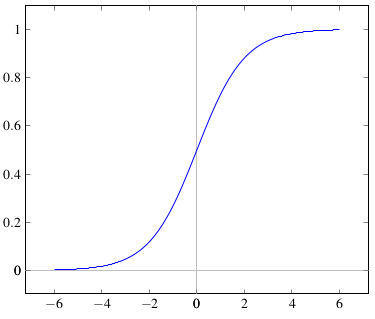
\includegraphics[width=2.5in]{sigmoid}} 
\hspace*{0.2in} % separation between the subfigures
\subfloat[Tanh] {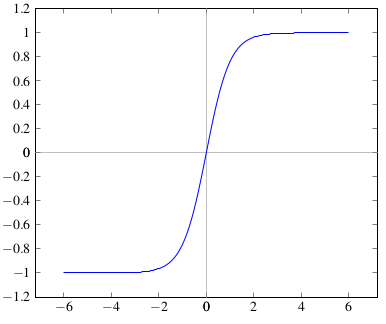
\includegraphics[width=2.5in]{tanh}}
\\
\subfloat[ReLU] {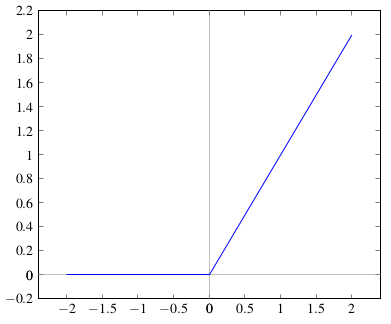
\includegraphics[width=2.5in]{relu}}
\hspace*{0.2in} % separation between the subfigures
\subfloat[LReLU] {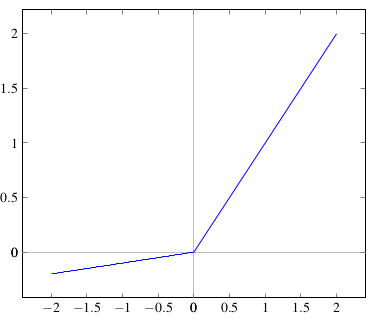
\includegraphics[width=2.5in]{lrelu}}


\caption{Neural network activation functions. } \label{fig:activation}
\end{figure}
\subsubsection{Sigmoid}
The sigmoid activation function is a non-linear function in the range of $]0, 1[$ and has the mathematical form defined in Equation \ref{eq:sigmoid} and is shown in the Figure \ref{fig:activation} (a).
\begin{equation}
f(x) = \frac{1}{1+e^{-x}}
\label{eq:sigmoid}
\end{equation}
It takes a real-valued number and transforms it to the range between 0 and 1. Small negative numbers become 0 and large positive numbers become 1. 
\subsubsection{Tanh}

The Hyperbolic Tangent (tanh) non-linearity is shown in Figure \ref{fig:activation} (b) and is defined in Equation \ref{eq:tanh}. It limits a real-valued number to the range of $[-1, 1]$. 
\begin{equation}
f(x) = \frac{e^x - e^{-x}}{e^x + e^{-x}}
\label{eq:tanh}
\end{equation}

\subsubsection{Rectified Linear Unit}

The Rectified Linear Unit (ReLU) has become very popular in the last few years and was one of the main discoveries that enabled the training of deeper neural networks. It computes the function 
\begin{equation}
f(x)=max \: (0,x)
\label{eq:relu}
\end{equation}
in other words, the activation is simply thresholded at zero, see Figure \ref{fig:activation} (c). 

\subsubsection{Leaky Rectified Linear Units}

Leaky Rectified Linear Units (LReLU) is an attempt to improve the ReLU. Instead of the function being zero when $x < 0$, a leaky ReLU will instead have a small negative slope (around 0.01). The function computes

\begin{equation}
f(x)=\begin{cases}
      \alpha x, & \text{if}\ x < 0\\
      x, & \text{otherwise}
    \end{cases}
\label{eq:lrelu}
\end{equation}

where $\alpha$ is a small constant, see Figure \ref{fig:activation} (d). 


\section{Deep Neural Networks}
Deep architectures are characterized by the multiple levels of non-linear operations
contained on a neural network. While many of the early successful applications of neural networks used shallow architectures (up to 3 hidden layers). It was found, however, that the mammal brain is organized in a deep architecture. The brain appears to process information through multiple stages, which is particularly clear in the primate visual system \cite{bengio2009learning}. 

It was observed in many experiments that deep networks are harder to train than shallow networks, and that training deep networks often get stuck in apparent local minima (or plateaus) when starting with random initialization of the network parameters. Deep Neural Networks have been investigated for decades, but training deep networks consistently yielded poor results. 

The proposal of the Convolutional Neural Network \cite{lecun1995convolutional} and some recent theoretical discoveries made training deep neural networks feasible. The CNN is a particular type of deep, feedforward neural network that is easier to train and generalized better than networks with full connectivity between adjacent layers \cite{lecun2015deep}. Besides, the theoretical findings include unsupervised training of the layers \cite{hinton2006fast}, Rectifier Linear Unit (ReLU) \cite{nair2010rectified} as the activation function and the regularization techniques Dropout \cite{srivastava2014dropout} and Batch Normalization \cite{ioffe2015batch}. 


\section{Convolutional Neural Networks}
CNNs combine three architectural ideas: local receptive fields, shared
(tied) weights and spatial or temporal sub-sampling \cite{lecun1998gradient}. When trained with appropriate regularization, CNN achieves state-of-the-art performance
on visual object recognition and image classification tasks \cite{lecun2015deep}. The CNN is composed of several layers of trainable filters (convolutional layers) and local neighborhood pooling operations (pooling layers) stacked in an alternating sequence starting with the raw input images. To illustrate the concept, Figure \ref{lenet} shows an example of an architecture of a CNN, namely, the Lenet \cite{lecun1998gradient}, one of the first applications of the CNN used for handwriting recognition.

\begin{figure}[!htb]
\centering
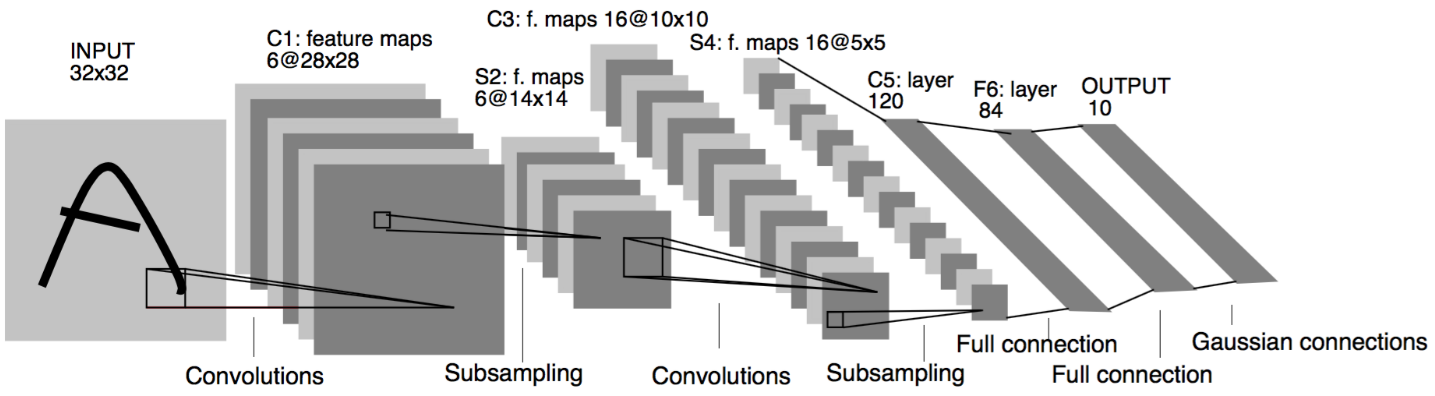
\includegraphics[width=\textwidth]{lenet}
\caption{Lenet \cite{lecun1998gradient}, a convolutional neural network used for handwriting recognition.}
\label{lenet}
\end{figure}

Figure \ref{learned} provides an example of the filters learned on a convolutional layer of a network trained for object classification, showing that this type of architecture is
capable of learning interesting feature detectors, similar to edge detectors.
\begin{figure}[!htb]
\centering
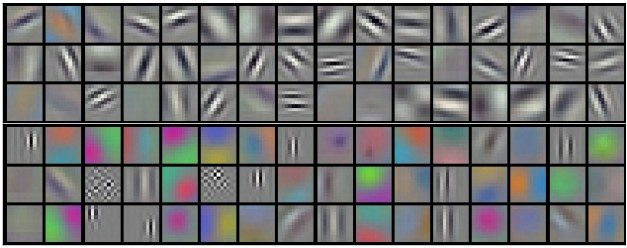
\includegraphics[width=0.7\textwidth]{learned}
\caption{Example of feature maps learned by the CNN proposed by \cite{krizhevsky2012imagenet} for object classification.}
\label{learned}
\end{figure}


\subsection{Convolutional Layer}
Convolutional layers have trainable filters (also called feature maps) that are applied
across the entire input \cite{lecun1995convolutional}. For each filter, each neuron is connected only to a subset of
the neurons in the previous layer. In the case of 2D input (such as images), the filters
define a small area (e.g., 3x3 or 5x5 pixels), and each neuron is connected only to the
nearby neurons (in this area) in the previous layer. The weights are shared across neurons,
leading the filters to learn frequent patterns that occur in any part of the image.

The definition for a 2D convolution layer is presented in Equation \ref{eq:cnn}. A 2D convolution layer is the application of a discrete convolution of the inputs $y^{(l-1)}$ with a filter $w^{(l)}$, adding a bias $b_{(l)}$ , followed by the application of an activation function $f$:

\begin{equation}
y^{(l)}_{rc} = f(\sum_{i=1}^{N_{r}} \sum_{j=1}^{N_{c}} y^{(l-1)}_{(r+i-1)(c+j-1)} w^{(l)}_{ij} + b^{(l)} )
\label{eq:cnn}
\end{equation}
where $y^{(l)}_{rc}$ is the output at position $\{r,c\}$, $N_{r}$ and $N_{c}$ are the number of rows and columns, respectively, of the 2D filter, $w^{(l)}_{ij}$ is the filter value at position $\{i,j\}$, $y^{(l-1)}_{(r+i-1)(c+j-1)}$ is the $\{r+i-1,c+j-1\}$.


The equation above is defined for all possible applications of the filter, as in Figure \ref{fig:convop} (a), that is, for
$r \in \{1, ..., I_{r} - N_{r} + 1\}$ and $c \in \{1, ..., I_{c} - N_{c} + 1\}$, where $I_{r}$ and $I_{c}$ are the number of rows and columns in the input to this layer. The convolutional layer can either apply the filters for all possible inputs \footnote{Animated representation can be found in: \url{https://raw.githubusercontent.com/vdumoulin/conv_arithmetic/master/gif/no_padding_no_strides.gif}}, or use a different strategy. Instead of applying the filter for all possible $\{r, c\}$ pairs, only the pairs with distance
$s$ are used, which is called the stride. A stride $s = 2$ \footnote{Animated representation of strides can be found in: \url{https://raw.githubusercontent.com/vdumoulin/conv_arithmetic/master/gif/no_padding_strides.gif}} is equivalent to apply the convolution for half of the possible pairs, as in Figure \ref{fig:convop} (b).

\begin{figure}[!htb]
\centering
\subfloat[Convolving a 3x3 kernel over a 4x4 input, with 1x1 stride.] {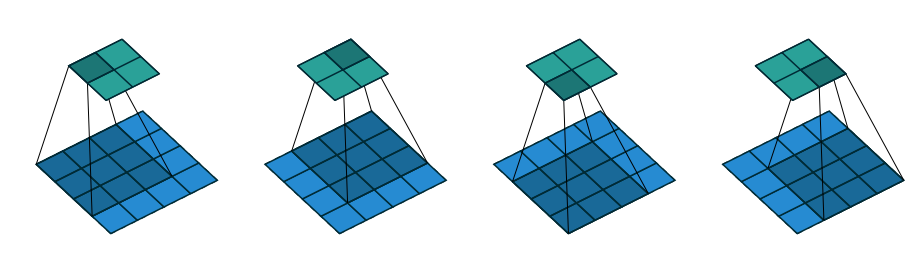
\includegraphics[width=\textwidth]{conv-operation}}
\\
\subfloat[Convolving a 3x3 kernel over a 5x5 input, with 2x2 stride.] {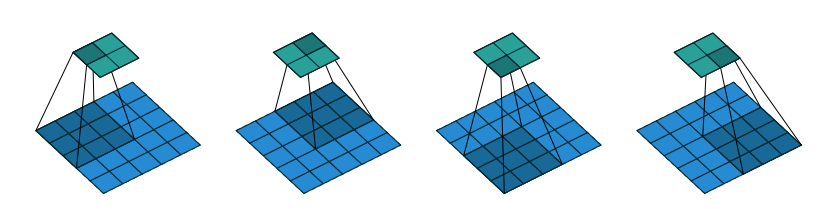
\includegraphics[width=\textwidth]{conv-operation-strides}}


\caption{Convolution operation with (a) stride 1x1 and (b) stride 2x2. Extracted from \cite{dumoulin2016guide}.} \label{fig:convop}
\end{figure}


\section{Fully Convolutional Network Architecture}

The Fully Convolutional Network (FCN) \cite{long2015fully} is a CNN modified for dense
predictions. This architecture was developed under the observation that although a typical CNN is designed for spatial inputs, such as images, it normally discard spatial information in their fully connected layers (FC). 

FCNs are, thus, rooted in the observation that spatial filters, which are learned during the CNN training, are useful for extracting low-level features, but FC layers are needed to incorporate high-level reasoning. The main idea of the FCN architecture is to convert the FC layers of a CNN into convolutional layers, expecting that the network retains the ability to learn high-level information and at the same time preserve spatial information. The FCN becomes, therefore, ``fully convolutional'' by having end-to-end convolutional layers. 

While CNNs are typically built in a sequence of convolutional, pooling, and fully connected layers, FCN adds an expanding path built with a transposed convolutional layer \cite{long2015fully}. The expanding path recovers spatial information by merging features skipped from the various resolution levels on the contracting path.

Unlike a CNN, which learns a general, nonlinear function that characterizes the input, FCNs learn an end-to-end nonlinear mapping from one input image to another. Because pixel-wise prediction is used, the label space is also transformed from a scalar to a two-dimensional image, where each pixel value represents the object class of its corresponding input pixel. An FCN with an input image and label is illustrated in Figure \ref{fcn-arch}


\begin{figure}[!htb]
\centering
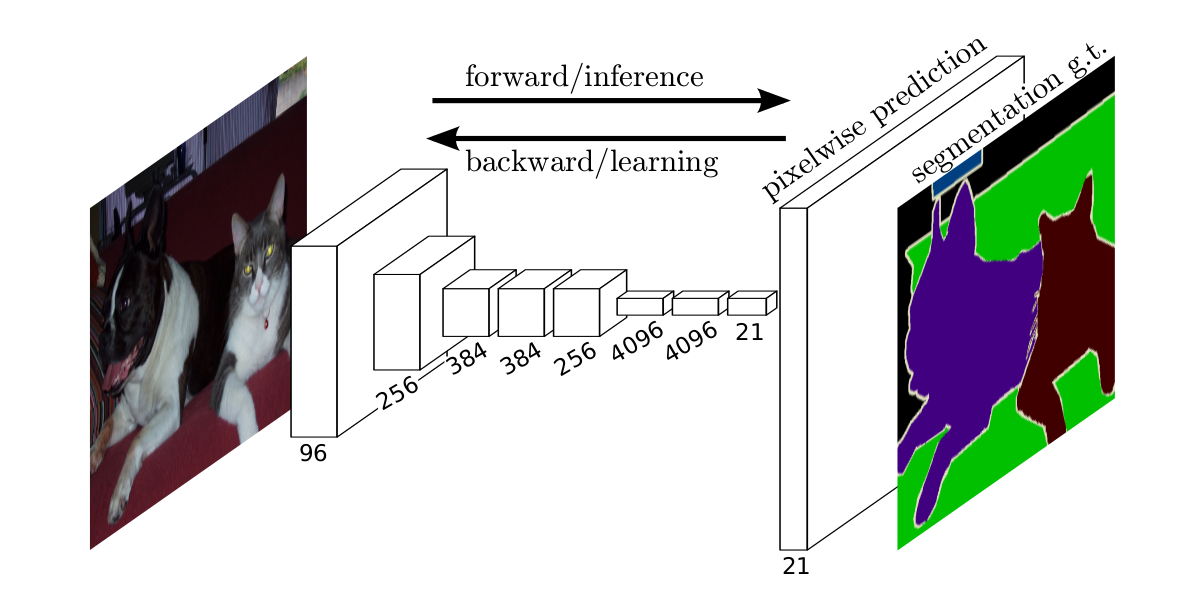
\includegraphics[width=\textwidth]{fcn-arch}
\caption{Fully convolutional networks can efficiently learn to make dense predictions for
per-pixel tasks. Extracted from \cite{long2015fully}}
\label{fcn-arch}
\end{figure}

\subsection{Transposed Convolution}
%https://arxiv.org/pdf/1603.07285.pdf p 19

Transposed convolutions - also called deconvolution or backward convolution - work by swapping the forward and backward passes of a convolution. One way to put it is to note that the kernel defines a convolution, but whether it is a direct convolution or a transposed convolution is determined by how the forward and backward passes are computed \cite{dumoulin2016guide}.

For instance, one might use such a transformation as the decoding layer of an FCN or project feature maps to a higher-dimensional space. Figure \ref{fig:transposed} illustrates the general backwards convolution process \cite{dumoulin2016guide}.

\begin{figure}[!htb]
\centering
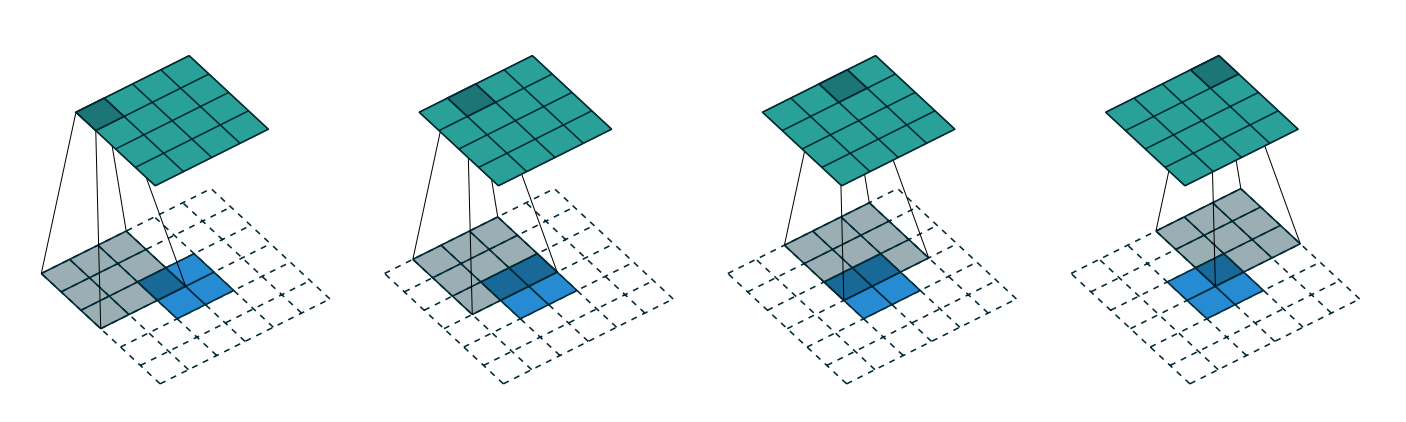
\includegraphics[width=\textwidth]{transposed}

\caption{Upsampling with transposed convolutions. Upsampling is done by padding
(white) the original pixels (blue) and convolving them with a filter (gray). The result is
an upsampled image (green). Here a stride of one is used, illustrated from left to right. Extracted from \cite{dumoulin2016guide}.} \label{fig:transposed}
\end{figure}

\section{Deep Neural Networks Training}

\subsection{Weight Initialization}
When the training of the neural network starts, the initial values of the weights and biases need to be provided. Some techniques to weight initialization have been proposed and shown to be useful to smooth the model convergence.

\subsubsection{Uniform}
The uniform initialization is the most simple. The model parameters are initialized through a random distribution in the range of $[l1, l2]$, where $l1$ and $l2$ are two constants.

\subsubsection{Glorot}
This weight initialization technique was proposed in \cite{glorot2010understanding}. The dynamic of the activation functions and the gradients weights were studied, and they found the neural network converges faster using the weight initialization described in Equation \ref{eq:glorot}.

\begin{equation}
W \sim U \; \left[\sqrt{\frac{6}{f_{in}+f_{out}}}\; \right] 
\label{eq:glorot}
\end{equation}
where $W$ are the weights, $U$ is an uniform distribution, and $f_{in}$ and $f_{out}$ are the number of units in the previous layer and the next layer, respectively.

\subsection{Optimization Algorithms}
Training the network consists in minimizing the error function, based on the gradients of the parameters with relation to the cost function, by updating the weights and biases, expecting that the network learns how to perform the task it is being trained for.

\subsubsection{Stochastic Gradient Descent}

The Stochastic Gradient Descent (SGD) algorithm, as defined in \cite{bishop2006pattern} can be summarized a series of iterations over mini-batches of the dataset, performing forward-propagation
followed by a back-propagation to calculate the error derivatives with respect to the parameters. The weights are updated using these derivatives, and a new mini-batch is used. This procedure is repeated until a convergence criterion is  reached. Common convergence criteria are a maximum number of epochs (number of times that the whole training set was used); a desired value for the cost function is reached, or training until the cost function shows no improvement in a number of iterations.

\subsubsection{Adaptive Moment Estimation}
The Adaptive Moment Estimation (ADAM) \cite{kingma2014adam} is a stochastic optimization method that can adaptively tune the learning rate per parameter and also keeps an exponentially decaying average of past gradients $m_t$ and $v_t$:

\begin{subequations}
\begin{gather}
\label{adamfirst}
m_t = \beta_1 m_{t-1} + (1 - \beta_1) g_t \\   
v_t = \beta_2 v_{t-1} + (1 - \beta_2) g_t^2  
\end{gather}
\end{subequations}
where $m_t$ and $v_t$ are estimates of the first moment and the second moment of the gradients respectively, $\beta_1$ and $\beta_2$ are the decay rate and $g$ is the gradient with respect to $w$. 

The authors observed that the moments are biased towards zero, especially during the initial time steps. They work around these biases by computing bias-corrected estimates:
\begin{subequations}
\begin{gather}
\hat{m}_t=\dfrac{m_t}{1 - \beta^t_1} \\
\hat{v}_t=\dfrac{v_t}{1 - \beta^t_2}
\label{adamend}
\end{gather}
\end{subequations}
Then, they use these computed variables to update the parameters:
\begin{equation}
w_{t+1} = w_{t} - \alpha \dfrac{\hat{m}_t}{\sqrt{\hat{v}_t} + \epsilon} 
\label{adamend2}
\end{equation}
The authors propose default values of 0.9 for $\beta_1$, 0.999 for $\beta_2$, and $10^{-8}$ for $\epsilon$.


